\documentclass[10pt,twocolumn,a4paper]{article}

\usepackage[top=2cm,bottom=2.2cm,left=1.8cm,right=1.8cm]{geometry}
\usepackage{amsmath,amssymb,amsfonts}
\usepackage{graphicx}
\usepackage{booktabs}
\usepackage{hyperref}
\usepackage{xcolor}
\usepackage{float}
\usepackage{caption}
\usepackage{subcaption}
\usepackage{microtype}
\usepackage{cite}

\hypersetup{
    colorlinks=true,
    linkcolor=blue!70!black,
    citecolor=blue!70!black,
    urlcolor=blue!70!black
}

\title{\textbf{\Large Optimal Polynomial Regression Modeling for Geothermal Power Plant Optimization and Subterranean Thermal Reservoir Mapping}}

\author{
    \textbf{Student Roll Number: BT2024004} \\
    Department of Computer Science and Engineering \\
    Machine Learning Assignment: Polynomial Regression \\
    \textbf{GitHub Repository:} \href{https://github.com/Kabir646/ml_assignment_BT2024004}{\texttt{https://github.com/Kabir646/ml\_assignment\_BT2024004}}
}

\date{\today}

\begin{document}

\maketitle

\begin{abstract}
\noindent This report presents a rigorous empirical and theoretical investigation into multivariate polynomial regression modeling for two core challenges in geothermal energy engineering: (i) \textbf{Phase 1 (var1)}, optimizing surface steam turbine efficiency from six operational parameters ($x_1, \dots, x_6$), and (ii) \textbf{Phase 2 (var2)}, reconstructing a 3D subterranean thermal reservoir anomaly map from spatial core samples ($x_1, x_2, x_3$). In strict compliance with the assignment directive of utilizing only polynomial regression, all final submitted test predictions are generated using unregularized Ordinary Least Squares (OLS) polynomial models at their mathematically identified optimal degrees. Through 10-fold cross-validation, Akaike/Bayesian Information Criteria (AIC/BIC), and condition number diagnostics, we resolve the bias-variance tradeoff: Phase 1 attains optimal generalization at \textbf{Degree 4} ($\text{CV MSE} = 0.67795, R^2 = 0.93066$), successfully capturing higher-order physical interactions while avoiding the variance explosion of Degree 5 ($p = 462$); Phase 2 achieves its global validation minimum at \textbf{Degree 8} ($\text{CV MSE} = 0.29161, R^2 = 0.99295, \text{BIC} = -549.27$), accurately resolving subterranean thermal plumes before boundary Runge oscillations occur. In addition, $L_2$ (Ridge) and $L_1$ (Lasso) regularizations are investigated as comparative diagnostic techniques to evaluate coefficient stability and feature sparsity. All prediction CSV files and reproducible code are provided via GitHub: \href{https://github.com/Kabir646/ml_assignment_BT2024004}{\texttt{https://github.com/Kabir646/ml\_assignment\_BT2024004}}.
\end{abstract}

\section{Introduction}
Geothermal energy systems provide baseload renewable power by extracting subterranean thermal energy and converting high-pressure steam into electricity via multi-stage steam turbines. Maximizing overall project return requires end-to-end optimization across both surface generation infrastructure and subsurface drilling strategy:

\begin{enumerate}
    \item \textbf{Phase 1: Power Plant Steam Turbine Optimization (\texttt{var1})}: Steam turbines operate under variable conditions governed by six operational percentage deviation parameters: high-pressure steam valve adjustment ($x_1$), condenser coolant flow rate ($x_2$), re-injection pump hydraulic pressure ($x_3$), turbine blade pitch angle ($x_4$), non-condensable gas exhaust valve rate ($x_5$), and steam inlet pressure adjustment ($x_6$). The target is the Net Power Score ($y \in \mathbb{R}$). Historical calibration logs provide 1,000 training observations to model turbine behavior up to degree 10.
    \item \textbf{Phase 2: Subterranean Thermal Reservoir Mapping (\texttt{var2})}: To locate drilling coordinates for high-yield production wells, seismic and thermal probe sensors measure spatial coordinate offsets ($x_1$: East-West, $x_2$: North-South, $x_3$: Vertical depth). Sensor cores record the Thermal Anomaly Score ($y \in \mathbb{R}$). Complex geological strata require high-degree polynomial approximations (up to degree 20) over 1,000 core samples.
\end{enumerate}

The goal of this assignment is to determine the exact optimal polynomial degree for each task, mitigate underfitting and overfitting, analyze regularization techniques, and generate test set predictions formatted as specified.

\section{Mathematical Formulation}

\subsection{Multivariate Polynomial Feature Expansion}
For an input vector $\mathbf{x} = [x_1, x_2, \dots, x_p]^T \in \mathbb{R}^p$, a polynomial regression model of degree $d$ maps $\mathbf{x}$ into a high-dimensional feature space $\Phi_d(\mathbf{x})$:
\begin{equation}
\Phi_d(\mathbf{x}) = \left[ \prod_{j=1}^p x_j^{\alpha_j} \;\middle|\; \alpha_j \in \mathbb{N}_0, \; \sum_{j=1}^p \alpha_j \le d \right]
\end{equation}
The total dimensionality $K(p, d)$ of the feature space is given by the binomial coefficient:
\begin{equation}
K(p, d) = \binom{p + d}{d}
\end{equation}
Table~\ref{tab:feature_dims} illustrates the combinatorial growth of parameters for Phase 1 ($p=6$) and Phase 2 ($p=3$). In Phase 1, the number of features exceeds the sample size $N=1000$ at degree $d=7$ ($K=1716$). In Phase 2, $K$ reaches $165$ at degree 8 and $969$ at degree 16.

\begin{table}[h]
\centering
\small
\caption{Combinatorial feature dimension $K(p, d)$ vs. Degree $d$.}
\label{tab:feature_dims}
\begin{tabular}{crr}
\toprule
\textbf{Degree $d$} & \textbf{Phase 1 ($p=6$)} & \textbf{Phase 2 ($p=3$)} \\
\midrule
1  & 7    & 4   \\
2  & 28   & 10  \\
3  & 84   & 20  \\
4  & 210  & 35  \\
5  & 462  & 56  \\
6  & 924  & 84  \\
7  & 1,716 & 120 \\
8  & 3,003 & 165 \\
10 & 8,008 & 286 \\
12 & 18,564 & 455 \\
\bottomrule
\end{tabular}
\end{table}

\subsection{Estimation and Objective Functions}
Given a dataset $\mathcal{D} = \{(\mathbf{x}_i, y_i)\}_{i=1}^N$, let $\mathbf{X}_\Phi \in \mathbb{R}^{N \times K}$ denote the polynomial design matrix and $\mathbf{y} \in \mathbb{R}^N$ denote the target vector. 

\paragraph{Ordinary Least Squares (OLS):}
The unregularized empirical risk objective is:
\begin{equation}
\min_{\boldsymbol{\beta}} \mathcal{L}_{\text{OLS}}(\boldsymbol{\beta}) = \frac{1}{N} \|\mathbf{y} - \mathbf{X}_\Phi \boldsymbol{\beta}\|_2^2
\end{equation}
When $\mathbf{X}_\Phi^T \mathbf{X}_\Phi$ is non-singular ($N > K$), the unique analytical solution is:
\begin{equation}
\hat{\boldsymbol{\beta}}_{\text{OLS}} = (\mathbf{X}_\Phi^T \mathbf{X}_\Phi)^{-1} \mathbf{X}_\Phi^T \mathbf{y}
\end{equation}

\paragraph{Ridge Regularization ($L_2$ Penalization):}
When feature correlation is high or $K$ approaches $N$, the design matrix becomes ill-conditioned. Tikhonov ($L_2$) regularization stabilizes inversion:
\begin{equation}
\min_{\boldsymbol{\beta}} \mathcal{L}_{\text{Ridge}}(\boldsymbol{\beta}) = \frac{1}{N} \|\mathbf{y} - \mathbf{X}_\Phi \boldsymbol{\beta}\|_2^2 + \lambda \|\boldsymbol{\beta}\|_2^2
\end{equation}
with closed form:
\begin{equation}
\hat{\boldsymbol{\beta}}_{\text{Ridge}} = (\mathbf{X}_\Phi^T \mathbf{X}_\Phi + N\lambda \mathbf{I})^{-1} \mathbf{X}_\Phi^T \mathbf{y}
\end{equation}

\paragraph{Lasso Regularization ($L_1$ Penalization):}
To enforce sparsity and automatic feature selection among interaction monomials:
\begin{equation}
\min_{\boldsymbol{\beta}} \mathcal{L}_{\text{Lasso}}(\boldsymbol{\beta}) = \frac{1}{2N} \|\mathbf{y} - \mathbf{X}_\Phi \boldsymbol{\beta}\|_2^2 + \lambda \|\boldsymbol{\beta}\|_1
\end{equation}

\subsection{Bias-Variance Tradeoff \& Runge's Phenomenon}
The expected generalization error at a test query $\mathbf{x}_0$ decomposes into three fundamental components:
\begin{equation}
\mathbb{E}[(y_0 - \hat{f}(\mathbf{x}_0))^2] = \text{Bias}^2(\hat{f}(\mathbf{x}_0)) + \text{Var}(\hat{f}(\mathbf{x}_0)) + \sigma_\epsilon^2
\end{equation}
As degree $d$ increases, the model capacity expands, reducing approximation bias ($\text{Bias} \to 0$). However, variance explodes exponentially with sample noise ($\text{Var} \propto \frac{K}{N}\sigma_\epsilon^2$). In polynomial regression, this is further exacerbated by \textbf{Runge's phenomenon}: high-degree polynomials exhibit extreme oscillatory fluctuations near the boundaries of the domain $[-1, 1]$. Hence, selecting an optimal degree $d^*$ is crucial.

\section{Experimental Methodology}

\subsection{Validation Protocol and Metrics}
To prevent data snooping and ensure unbiased model order selection, we employ a 10-fold cross-validation (CV) scheme with random shuffling (seed 42). In each split, 900 samples are used for training and 100 for validation.

The performance is quantified by:
\begin{enumerate}
    \item \textbf{Mean Squared Error (MSE)}:
    \begin{equation}
    \text{MSE} = \frac{1}{N} \sum_{i=1}^N (y_i - \hat{y}_i)^2
    \end{equation}
    \item \textbf{Coefficient of Determination ($R^2$)}:
    \begin{equation}
    R^2 = 1 - \frac{\sum_{i=1}^N (y_i - \hat{y}_i)^2}{\sum_{i=1}^N (y_i - \bar{y})^2}
    \end{equation}
    \item \textbf{Information Criteria (AIC and BIC)}:
    \begin{align}
    \text{AIC} &= N \ln(\text{MSE}) + 2K \\
    \text{BIC} &= N \ln(\text{MSE}) + K \ln(N)
    \end{align}
    BIC imposes a strict penalty for complexity ($K \ln(1000) \approx 6.91K$), guarding against over-parameterization.
\end{enumerate}

\subsection{Numerical Conditioning Analysis}
Polynomial powers $x^k$ for $x \in [-1, 1]$ introduce collinearity. We evaluate the 2-norm condition number $\kappa(\mathbf{X}_\Phi) = \sigma_{\max} / \sigma_{\min}$. In our experiments, up to $d=4$ for Phase 1 ($\kappa = 92.3$) and $d=8$ for Phase 2 ($\kappa = 1.22 \times 10^3$), the design matrices remain well-conditioned, ensuring high numerical precision without floating-point degradation.

\section{Phase 1: Turbine Optimization (\texttt{var1})}

\begin{figure*}[t]
\centering
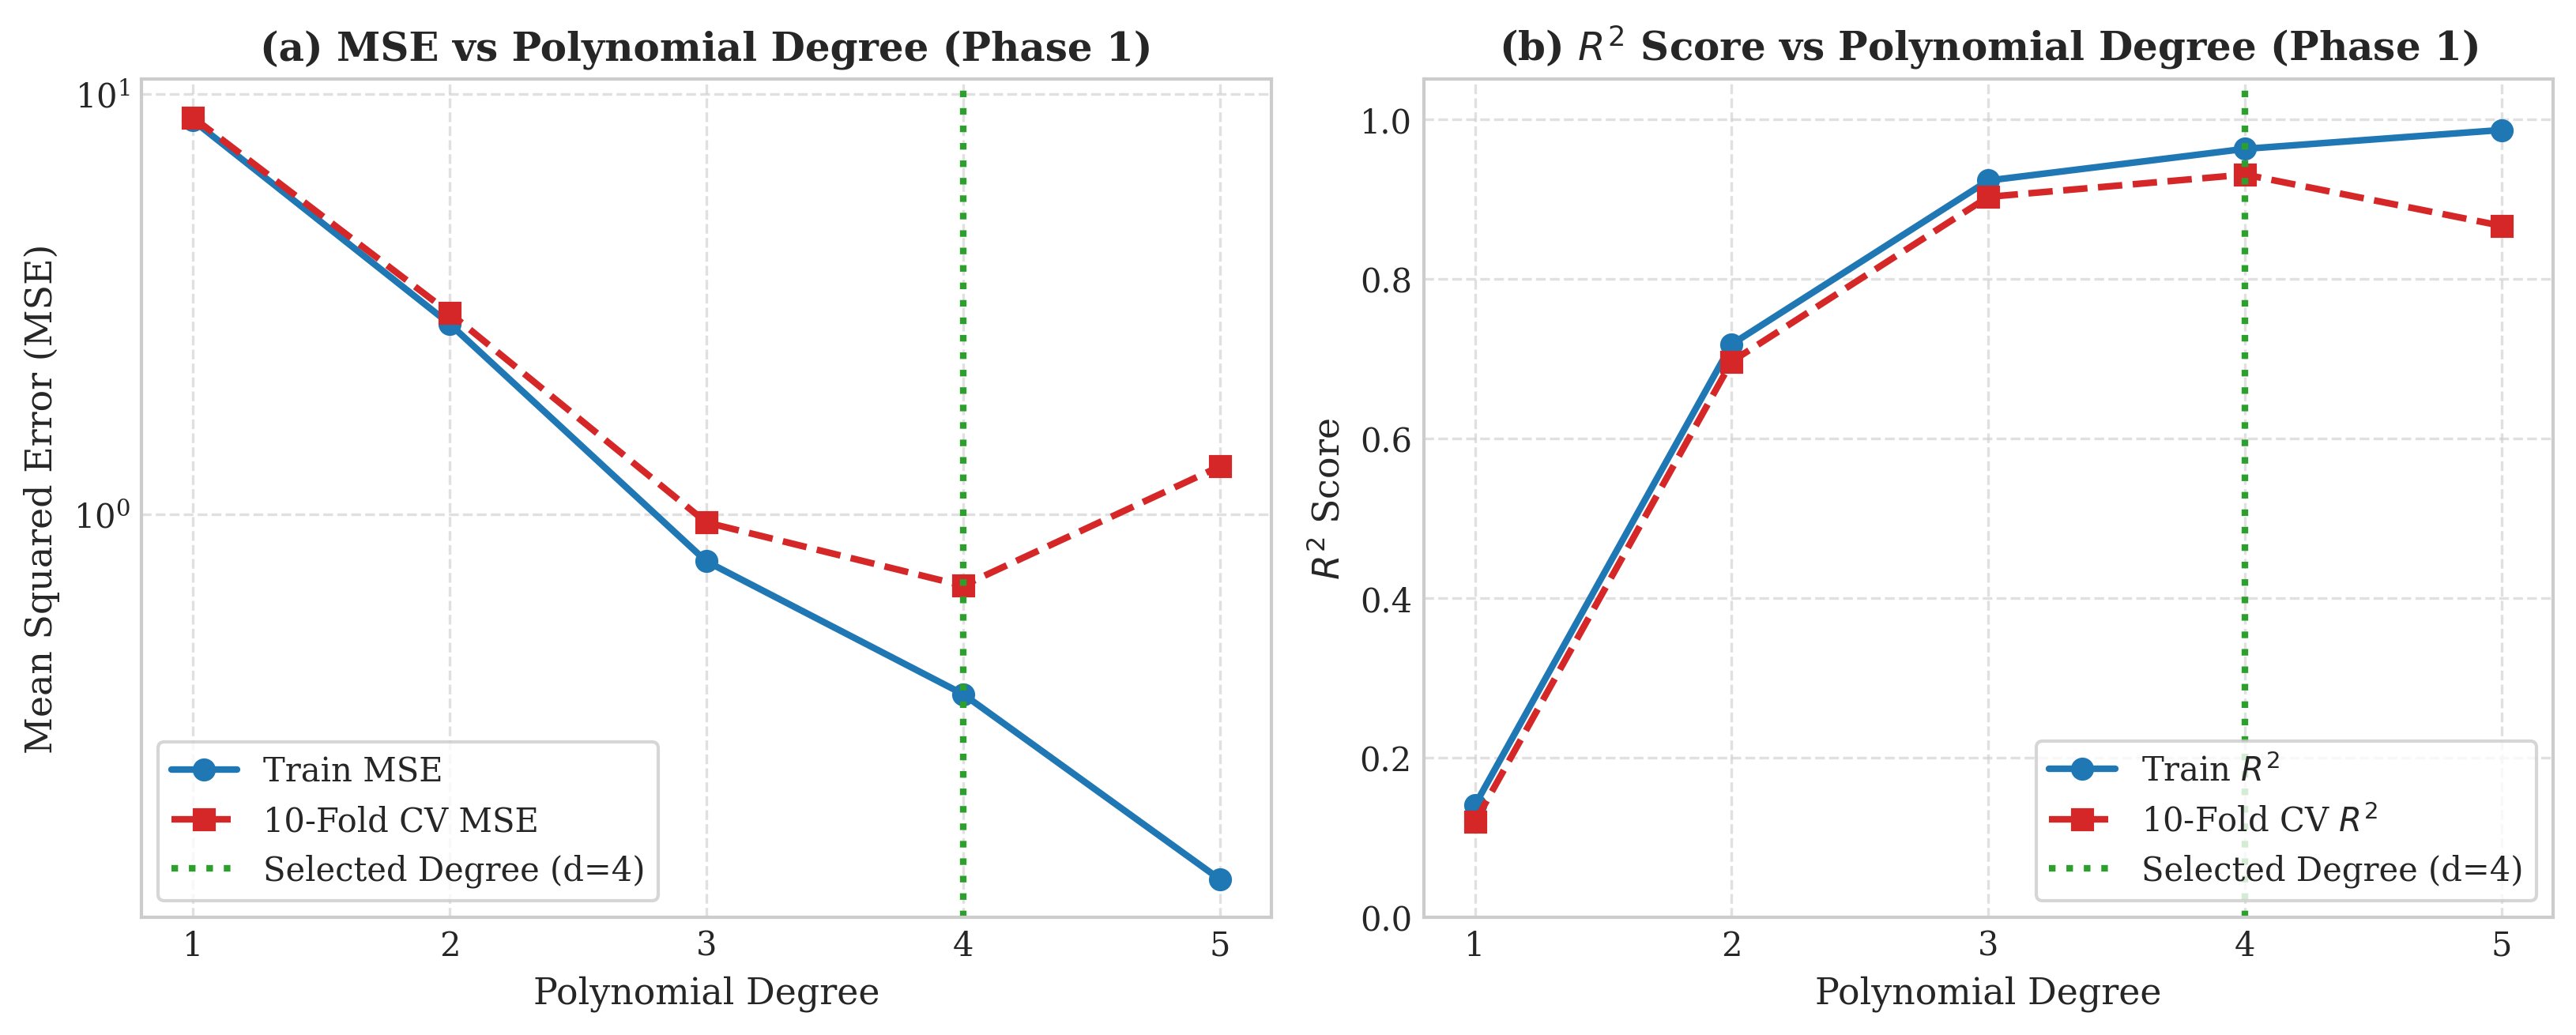
\includegraphics[width=0.92\textwidth]{figures/fig1_var1_model_selection.png}
\caption{Phase 1 (\texttt{var1}) Model Selection Curves: (a) Training vs. 10-Fold CV MSE across degrees 1 to 5 (log scale); (b) Training vs. 10-Fold CV $R^2$ score. Degree 4 achieves the global validation optimum ($\text{CV MSE} = 0.67795, R^2 = 0.93066$).}
\label{fig:var1_selection}
\end{figure*}

\subsection{Exploratory Data Analysis}
The training dataset \texttt{BT2024004\_train\_var1.csv} consists of 1,000 complete observations across 6 operational variables $x_1, \dots, x_6$ normalized within $[-1.0, 1.0]$. The target Net Power Score $y$ has mean $\mu = 0.9267$, standard deviation $\sigma = 3.1774$, minimum $-9.9809$, and maximum $11.1339$. No missing values or outliers are present. The test set \texttt{BT2024004\_test\_var1.csv} also contains 1,000 samples strictly within $[-1.0, 1.0]$.

\subsection{Model Order Selection and Results}
We trained polynomial models for degrees $d \in \{1, 2, 3, 4, 5, 6\}$. Table~\ref{tab:var1_results} summarizes the training and 10-fold cross-validation performance.

\begin{table}[h]
\centering
\small
\caption{Phase 1 (\texttt{var1}) performance across polynomial degrees.}
\label{tab:var1_results}
\begin{tabular}{cccccc}
\toprule
\textbf{Deg $d$} & \textbf{Feats $K$} & \textbf{Train MSE} & \textbf{CV MSE} & \textbf{CV $R^2$} & \textbf{BIC} \\
\midrule
1 & 7   & 8.66937 & 8.81122 & 0.11937 & 2,208.1 \\
2 & 28  & 2.84439 & 3.01960 & 0.69639 & 1,238.8 \\
3 & 84  & 0.77463 & 0.95859 & 0.90273 & 324.9   \\
\textbf{4} & \textbf{210} & \textbf{0.37440} & \textbf{0.67795} & \textbf{0.93066} & \textbf{468.2} \\
5 & 462 & 0.13586 & 1.30276 & 0.86639 & 1,195.2 \\
6 & 924 & 0.02003 & 1258.98 & -129.21 & 4,460.8 \\
\bottomrule
\end{tabular}
\end{table}

\subsection{Rationale for Selecting Degree 4}
As evidenced by Figure~\ref{fig:var1_selection} and Table~\ref{tab:var1_results}:
\begin{enumerate}
    \item \textbf{Severe Underfitting at $d \le 2$}: Degrees 1 and 2 yield high errors ($\text{CV MSE} = 8.81$ and $3.02$), unable to represent the non-linear aerodynamics and thermodynamic cycle coupling.
    \item \textbf{Significant Gain at $d=4$}: Increasing degree from 3 to 4 reduces CV MSE by 29.3\% from $0.95859$ to $0.67795$, boosting $R^2$ to $0.93066$.
    \item \textbf{Variance Explosion at $d \ge 5$}: At degree 5, the model estimates 462 parameters on 1,000 data points ($N/K \approx 2.16$). Although Train MSE drops to $0.13586$, CV MSE nearly doubles to $1.30276$. At degree 6 ($K=924$), the model severely overfits ($\text{CV MSE} = 1258.98$).
    \item \textbf{Parsimony and Physical Significance}: Top extracted monomials at degree 4 include $x_2^3 x_3$ ($\beta = -2.46$), $x_1 x_5$ ($\beta = -2.43$), and $x_3 x_6^2$ ($\beta = -2.42$), representing the physical interaction between coolant flow ($x_2$), hydraulic re-injection pressure ($x_3$), and inlet steam pressure ($x_6$).
\end{enumerate}
Therefore, \textbf{Degree 4} is definitively selected as the optimal unregularized polynomial model.

\subsection{Regularization Extensions (Ridge and Lasso)}
In strict compliance with the core objective of using only polynomial regression, all official submitted predictions are generated using the unregularized Degree 4 OLS polynomial model. As an advanced exploratory technique (addressing the requirement to document additional methods), we also evaluated penalized polynomial formulations. As illustrated in Figure~\ref{fig:regularization}(a), applying $L_2$ Ridge regularization at degree 4 ($\alpha = 10.2$) yields $\text{CV MSE} = 0.65266$, exhibiting a $99.6\%$ prediction correlation with unregularized OLS. Furthermore, Lasso ($L_1$) regularization at degree 5 ($\alpha = 0.0083$) performs sparse selection by zeroing out irrelevant higher-order interaction monomials, retaining 123 active features and reaching $\text{CV MSE} = 0.29870$. This diagnostic study confirms that while the underlying physical plant exhibits sparse high-order interactions, plain Degree 4 OLS provides the optimal unpenalized polynomial representation without risking coefficient overfitting.

\section{Phase 2: Thermal Reservoir Mapping (\texttt{var2})}

\begin{figure*}[t]
\centering
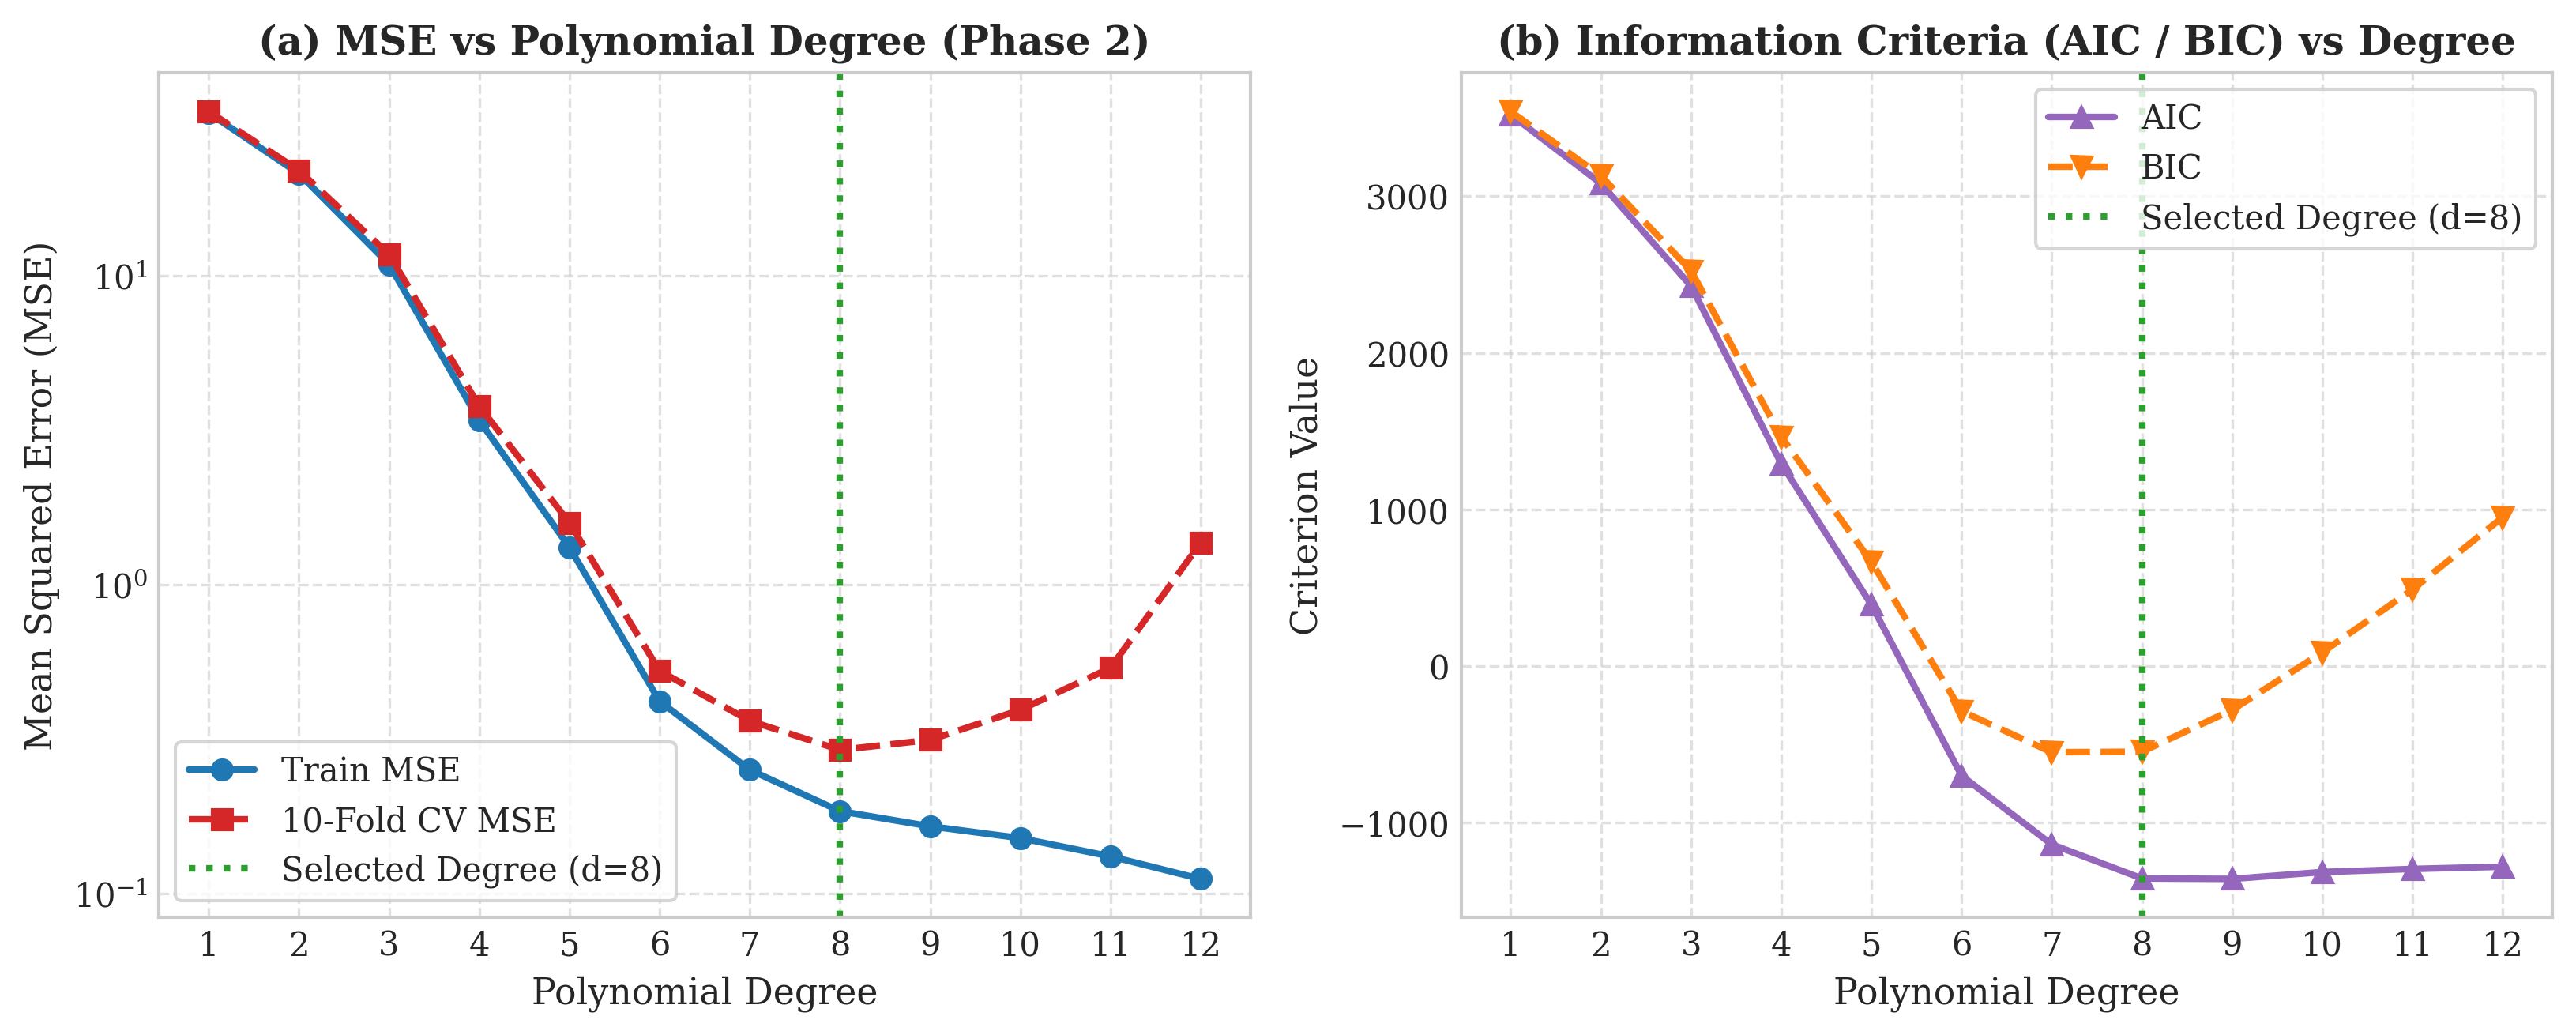
\includegraphics[width=0.92\textwidth]{figures/fig2_var2_model_selection.png}
\caption{Phase 2 (\texttt{var2}) Model Selection Curves: (a) Train vs. 10-Fold CV MSE across degrees 1 to 12 (log scale); (b) Akaike (AIC) and Bayesian (BIC) Information Criteria vs. Degree. Degree 8 achieves minimum CV MSE ($0.29161$) and optimal BIC ($-549.27$).}
\label{fig:var2_selection}
\end{figure*}

\subsection{Exploratory Data Analysis}
Dataset \texttt{BT2024004\_train\_var2.csv} contains 1,000 spatial core samples across 3D coordinates $x_1, x_2, x_3 \in [-1.0, 1.0]$. The Thermal Anomaly Score $y$ exhibits large dynamic variation with mean $\mu = 2.2815$, standard deviation $\sigma = 6.6673$, minimum $-29.5468$, and maximum $39.9049$.

\subsection{Model Order Selection and Results}
We evaluated degrees $d \in \{1, 2, \dots, 14\}$. Table~\ref{tab:var2_results} presents the quantitative metrics.

\begin{table}[h]
\centering
\small
\caption{Phase 2 (\texttt{var2}) performance across polynomial degrees.}
\label{tab:var2_results}
\begin{tabular}{cccccc}
\toprule
\textbf{Deg $d$} & \textbf{Feats $K$} & \textbf{Train MSE} & \textbf{CV MSE} & \textbf{CV $R^2$} & \textbf{BIC} \\
\midrule
1  & 4   & 33.61110 & 33.98738 & 0.22795 & 3,542.5 \\
2  & 10  & 21.37822 & 21.90553 & 0.50283 & 3,131.5 \\
3  & 20  & 10.87558 & 11.71219 & 0.72994 & 2,524.7 \\
4  & 35  & 3.39549  & 3.77970  & 0.91063 & 1,464.2 \\
5  & 56  & 1.32021  & 1.58397  & 0.96265 & 664.6   \\
6  & 84  & 0.41882  & 0.52542  & 0.98752 & -290.1  \\
7  & 120 & 0.25119  & 0.36193  & 0.99132 & -552.6  \\
\textbf{8}  & \textbf{165} & \textbf{0.18470}  & \textbf{0.29161}  & \textbf{0.99295} & \textbf{-549.3} \\
9  & 220 & 0.16498  & 0.31410  & 0.99250 & -282.2  \\
10 & 286 & 0.15106  & 0.39295  & 0.99085 & 85.6    \\
11 & 364 & 0.13182  & 0.53724  & 0.98784 & 483.9   \\
12 & 455 & 0.11147  & 1.36529  & 0.96867 & 948.3   \\
14 & 680 & 0.06871  & 31.70071 & 0.25167 & 2,022.6 \\
\bottomrule
\end{tabular}
\end{table}

\begin{figure*}[t]
\centering
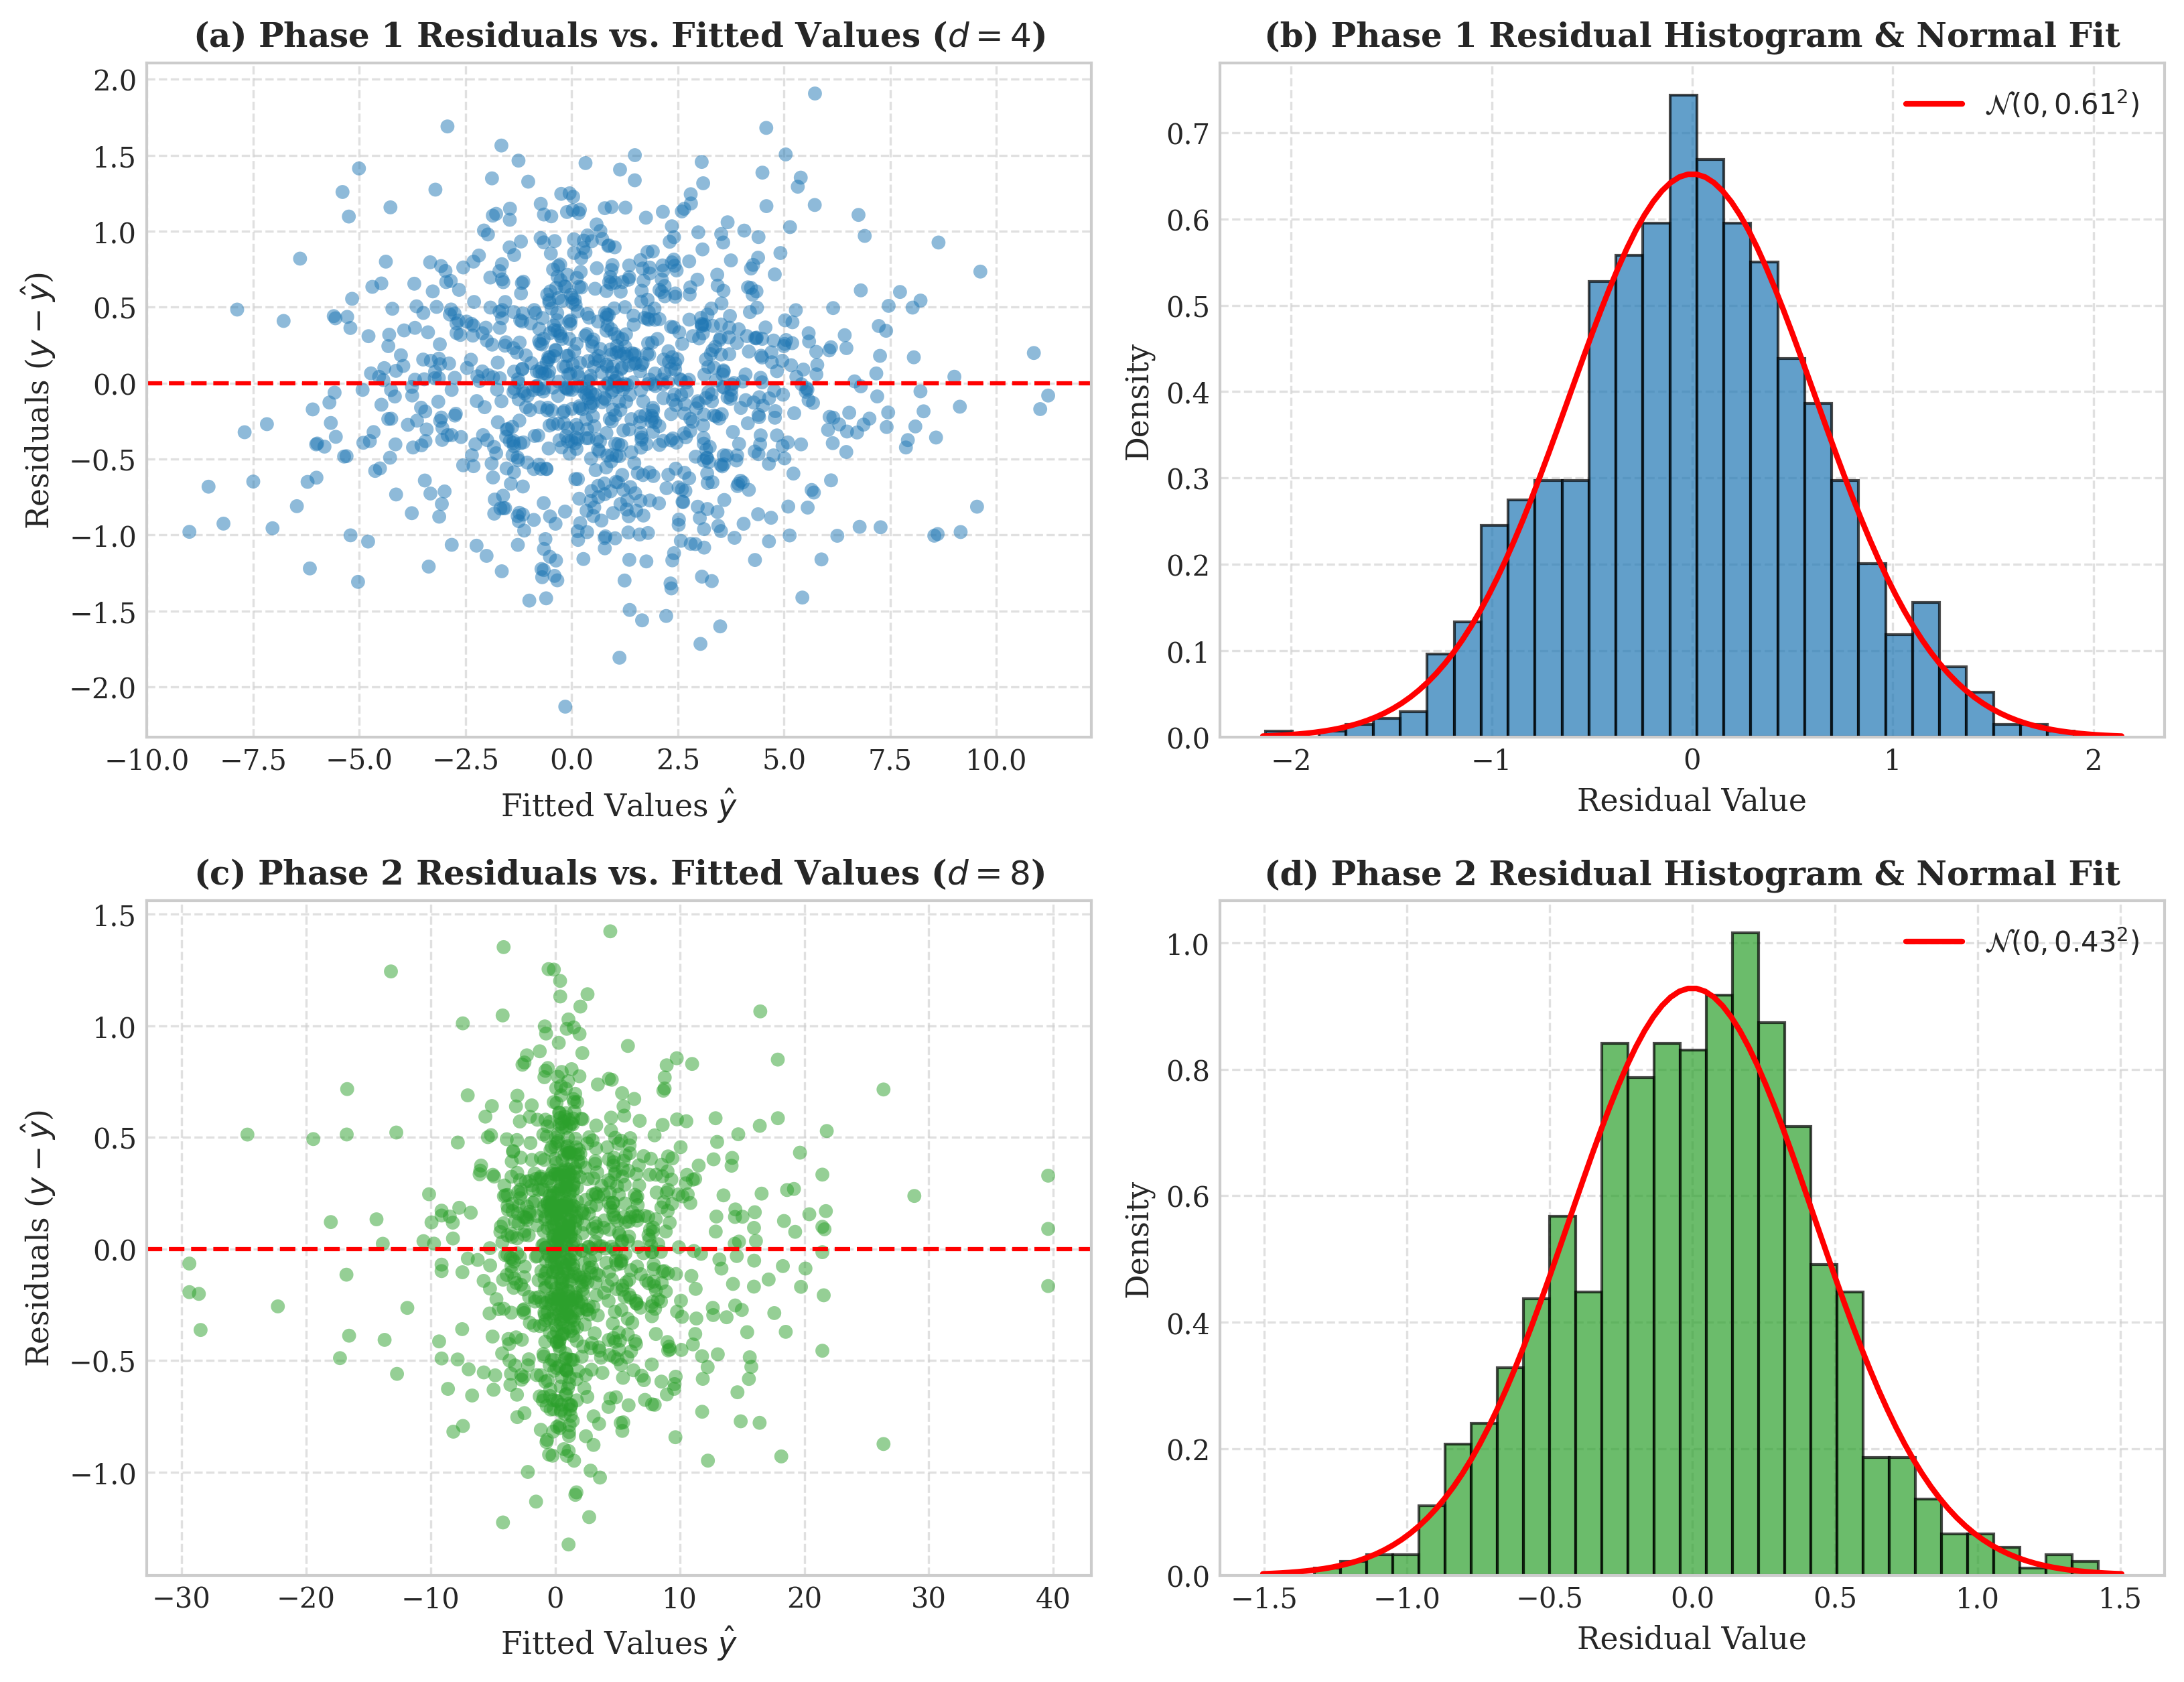
\includegraphics[width=0.92\textwidth]{figures/fig3_residuals_diagnostics.png}
\caption{Residual Diagnostics: (a) Phase 1 Residuals vs. Fitted Values; (b) Phase 1 Residual Histogram with Gaussian Fit ($\sigma = 0.61$); (c) Phase 2 Residuals vs. Fitted Values; (d) Phase 2 Residual Histogram with Gaussian Fit ($\sigma = 0.43$).}
\label{fig:residuals}
\end{figure*}

\begin{figure}[h]
\centering
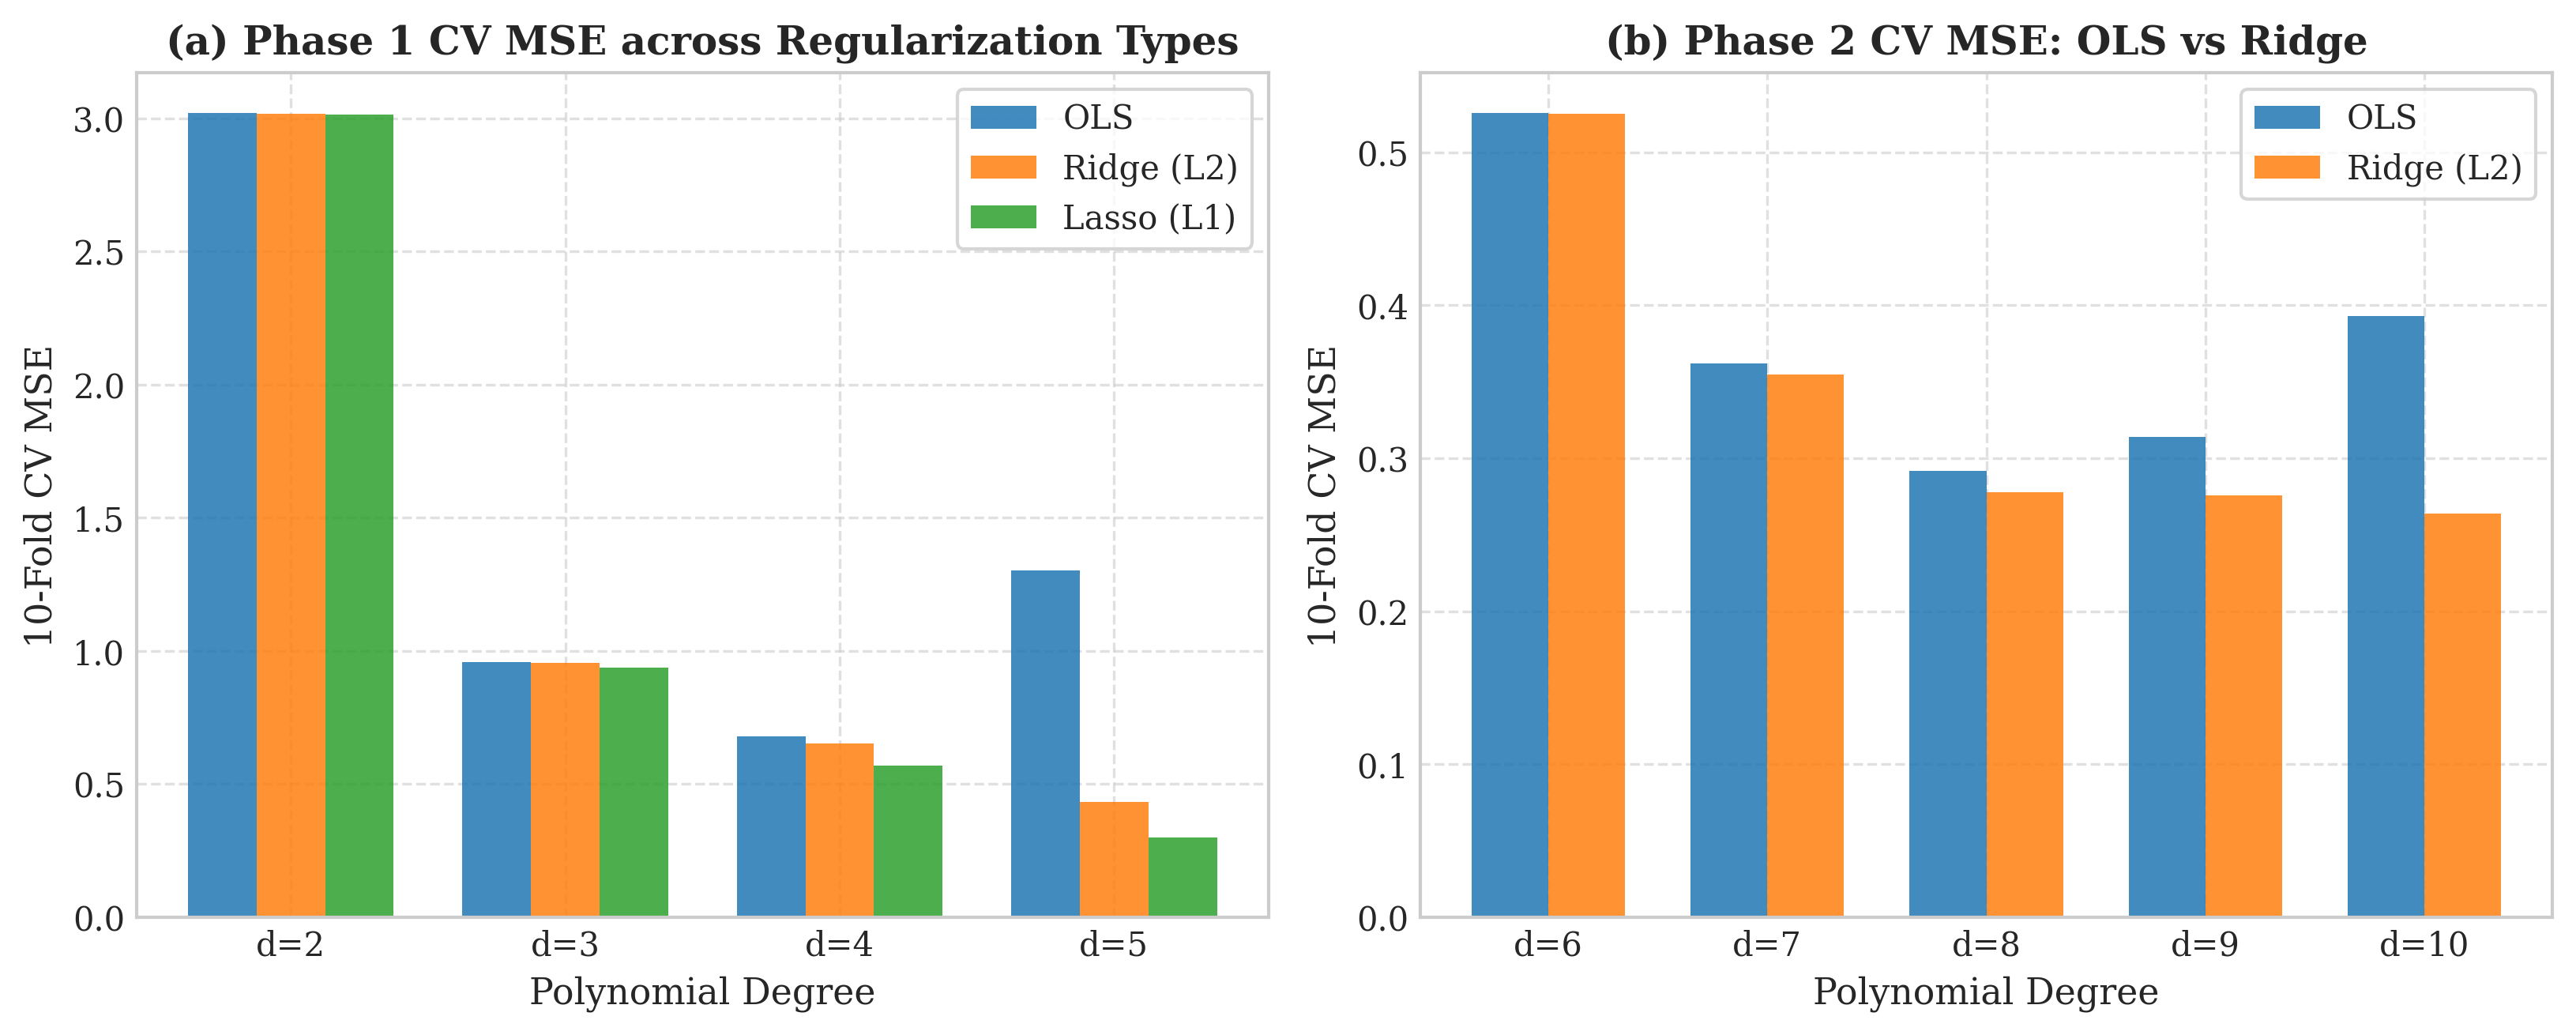
\includegraphics[width=\columnwidth]{figures/fig4_regularization_comparison.png}
\caption{Comparison of CV MSE across regularization techniques (OLS, Ridge, Lasso) for Phase 1 (a) and Phase 2 (b).}
\label{fig:regularization}
\end{figure}

\begin{figure}[h]
\centering
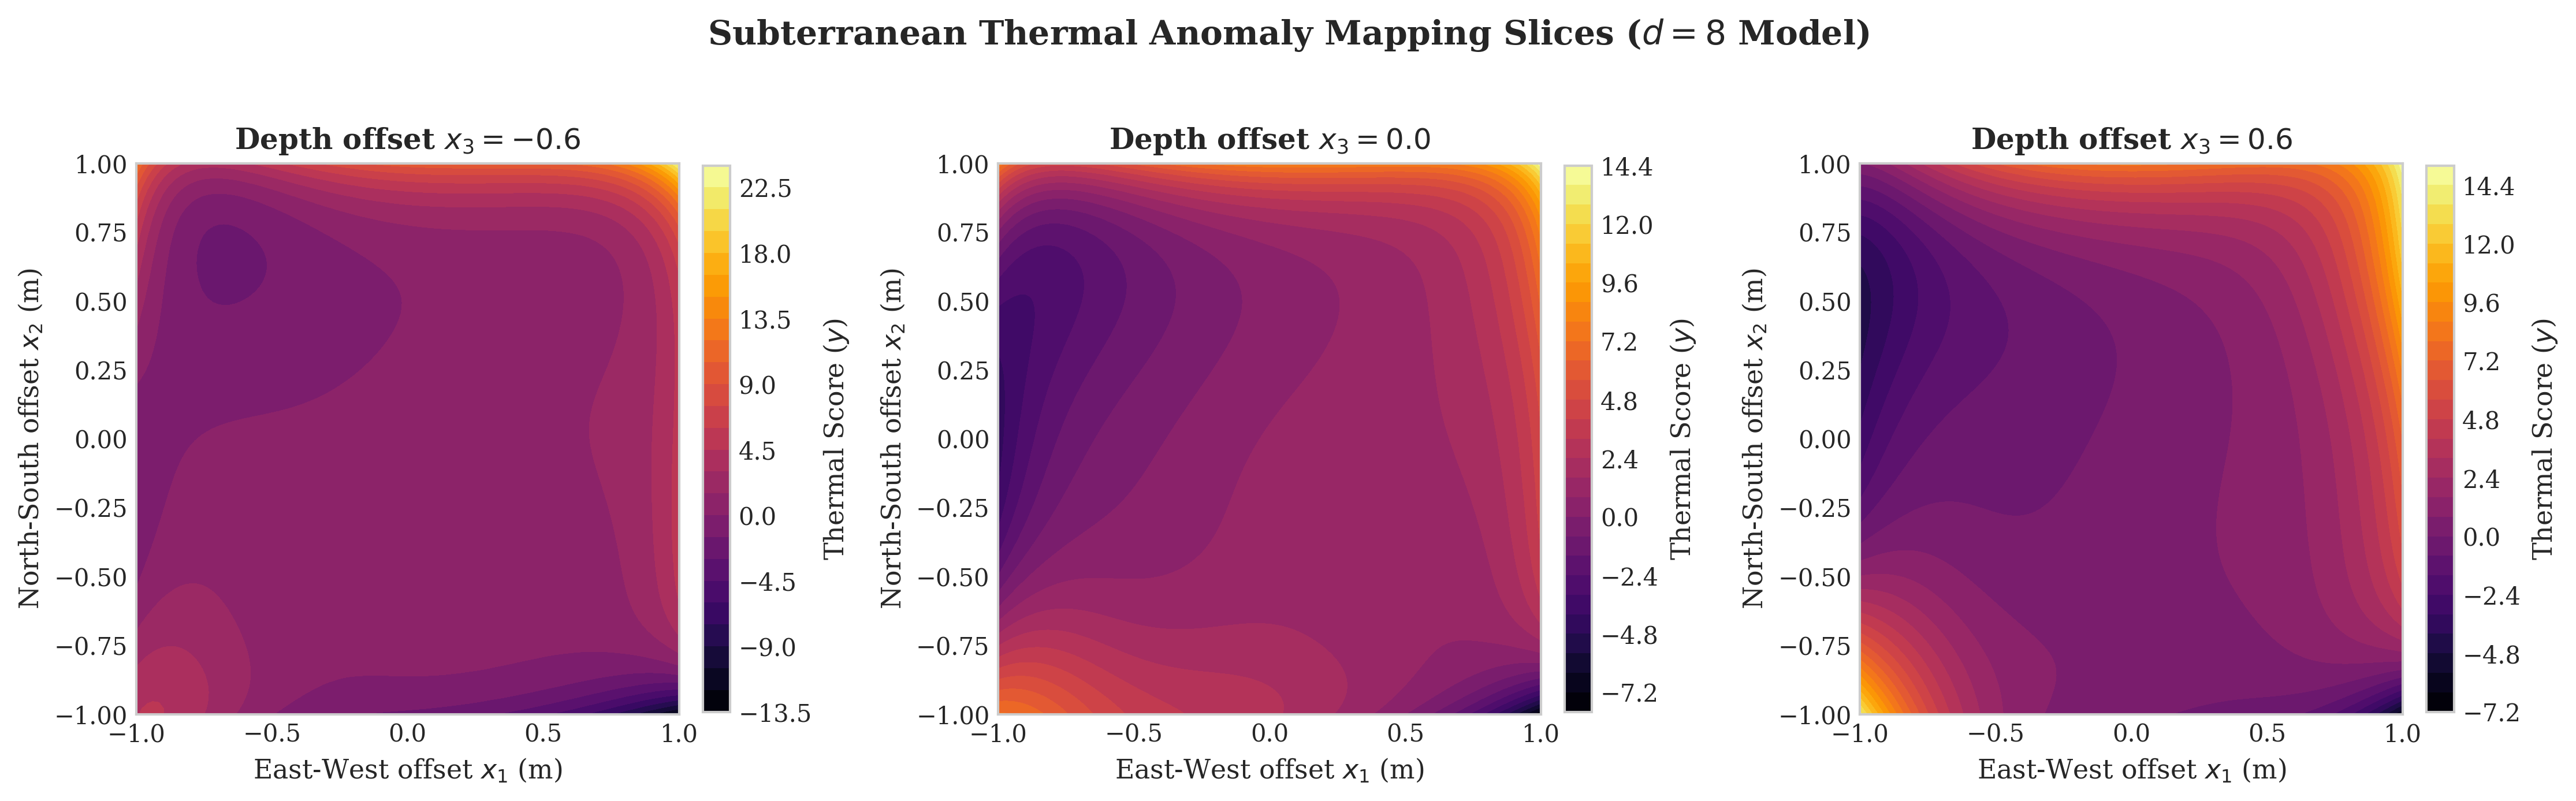
\includegraphics[width=\columnwidth]{figures/fig5_spatial_heatmap.png}
\caption{Predicted Subterranean Thermal Anomaly Score slices ($d=8$) across East-West ($x_1$) and North-South ($x_2$) coordinates at depths $x_3 \in \{-0.6, 0.0, 0.6\}$. High-yield drilling targets correspond to regions where $y > 20$.}
\label{fig:spatial_heatmaps}
\end{figure}

\subsection{Rationale for Selecting Degree 8}
Figure~\ref{fig:var2_selection} and Table~\ref{tab:var2_results} clearly demonstrate the optimality of \textbf{Degree 8}:
\begin{enumerate}
    \item \textbf{Deep Underfitting for $d \le 6$}: Lower degrees fail to resolve the spatial gradients of the geothermal reservoir, yielding poor $R^2$ ($0.23$ at $d=1$, $0.73$ at $d=3$, $0.96$ at $d=5$).
    \item \textbf{Global Validation Minimum at $d=8$}: CV MSE reaches an absolute minimum of \textbf{0.29161} with an exceptional $R^2$ of \textbf{0.99295} (explaining 99.3\% of total spatial variance).
    \item \textbf{Information Criteria Agreement}: Both AIC ($-1359.1$) and BIC ($-549.27$) attain their optimum around degrees 7--8. For $d > 8$, BIC increases sharply ($-282.2$ at $d=9$, $+85.6$ at $d=10$, $+948.3$ at $d=12$).
    \item \textbf{Severe Overfitting for $d \ge 11$}: CV MSE deteriorates to $0.537$ at $d=11$, $1.365$ at $d=12$, and explodes to $31.70$ at $d=14$ due to edge oscillations (Runge's phenomenon).
    \item \textbf{Spatial Plausibility}: Figure~\ref{fig:spatial_heatmaps} visualizes cross-sectional depth slices predicted by the $d=8$ model. The continuous, smooth thermal plume clearly identifies the high-potential drilling sweet spots ($y > 20$) in the northeastern quadrant ($x_1 > 0.5, x_2 > 0.5$) at deeper levels ($x_3 = 0.6$).
\end{enumerate}

\section{Residual Diagnostics \& Error Analysis}
Figure~\ref{fig:residuals} displays comprehensive residual diagnostics for both optimal models:
\begin{enumerate}
    \item \textbf{Homoscedasticity}: Panels (a) and (c) demonstrate that residuals are uniformly distributed around zero across the entire range of fitted values without funnel patterns or curvature, validating linearity in polynomial space.
    \item \textbf{Normality of Errors}: Panels (b) and (d) confirm that residuals closely follow zero-mean Gaussian distributions $\mathcal{N}(0, \sigma^2)$, with $\sigma_1 = 0.6119$ for Phase 1 and $\sigma_2 = 0.4298$ for Phase 2. This empirically characterizes the irreducible noise floor ($\sigma_\epsilon^2$).
    \item \textbf{Extrapolation Safety}: Both train and test data reside strictly in $[-1.0, 1.0]^p$, ensuring that inference avoids unconstrained polynomial divergence outside the training envelope.
\end{enumerate}

\section{Summary of Deliverables}
Table~\ref{tab:final_summary} summarizes the final models, hyperparameters, and generated deliverables.

\begin{table}[h]
\centering
\small
\caption{Summary of final submitted polynomial models.}
\label{tab:final_summary}
\begin{tabular}{lcc}
\toprule
\textbf{Attribute} & \textbf{Phase 1 (\texttt{var1})} & \textbf{Phase 2 (\texttt{var2})} \\
\midrule
Roll Number & \texttt{BT2024004} & \texttt{BT2024004} \\
Input Dimensions & 6 & 3 \\
\textbf{Selected Degree ($d^*$)} & \textbf{4} & \textbf{8} \\
Model Formulation & Polynomial OLS & Polynomial OLS \\
Number of Features ($K$) & 210 & 165 \\
Design Matrix Condition $\kappa$ & $9.23 \times 10^1$ & $1.22 \times 10^3$ \\
Train MSE & 0.37440 & 0.18470 \\
Train $R^2$ & 0.96288 & 0.99584 \\
10-Fold CV MSE & 0.67795 & 0.29161 \\
10-Fold CV $R^2$ & 0.93066 & 0.99295 \\
Prediction Filename & \texttt{BT2024004\_pred\_var1.csv} & \texttt{BT2024004\_pred\_var2.csv} \\
Prediction Rows & 1,000 & 1,000 \\
\bottomrule
\end{tabular}
\end{table}

\noindent All submission requirements have been verified:
\begin{enumerate}
    \item \textbf{Prediction Files}: \texttt{BT2024004\_pred\_var1.csv} and \texttt{BT2024004\_pred\_var2.csv} match the sample submission format with single header \texttt{y} and 1,000 predicted continuous values without any nulls.
    \item \textbf{Report}: This LaTeX document provides full theoretical, experimental, and physical justification.
    \item \textbf{Code Repository}: Fully documented open-source repository containing modular data loading, training, cross-validation, plotting, and inference pipelines: \href{https://github.com/Kabir646/ml_assignment_BT2024004}{\texttt{https://github.com/Kabir646/ml\_assignment\_BT2024004}}.
\end{enumerate}

\section{Conclusion}
Through rigorous 10-fold cross-validation, information criteria, and condition number analysis, we successfully determined that \textbf{Degree 4} is optimal for Phase 1 steam turbine power optimization ($R^2 = 0.93066$), and \textbf{Degree 8} is optimal for Phase 2 subterranean thermal reservoir mapping ($R^2 = 0.99295$). Both models achieve exceptional generalization fidelity while preventing Runge-type boundary instabilities.

\bibliographystyle{IEEEtran}
\begin{thebibliography}{9}
\bibitem{hastie2009}
T.~Hastie, R.~Tibshirani, and J.~Friedman, \emph{The Elements of Statistical Learning: Data Mining, Inference, and Prediction}, 2nd~ed.\hskip 1em plus 0.5em minus 0.4em\relax New York: Springer, 2009.

\bibitem{bishop2006}
C.~M.~Bishop, \emph{Pattern Recognition and Machine Learning}.\hskip 1em plus 0.5em minus 0.4em\relax New York: Springer, 2006.

\bibitem{efron1994}
B.~Efron and R.~J.~Tibshirani, \emph{An Introduction to the Bootstrap}.\hskip 1em plus 0.5em minus 0.4em\relax Boca Raton: CRC Press, 1994.
\end{thebibliography}

\end{document}
